% !TEX program = pdflatex
% ---------------------------------------------------------------------------
% Slide deck — first structural draft, oriented on Outline.tex
% Minimal skeleton: one section per outline section, frames to be populated
% step by step. Figures live in figures/, table fragments in tables/.
% ---------------------------------------------------------------------------
\documentclass[aspectratio=169,11pt]{beamer}

\usetheme{Madrid}
\usecolortheme{default}
\setbeamertemplate{navigation symbols}{}
\setbeamertemplate{caption}{\insertcaption}

\usepackage{booktabs}
\usepackage{siunitx}   % needed by the estout table fragments (S columns)
\usepackage{graphicx}
\graphicspath{{figures/}}

% --- Working title — adjust freely -----------------------------------------
\title[HF sovereign basis trading]{Hedge Funds in the Sovereign Cash--Futures Trade:\\ Anatomy and Fragility}
\author{Felix Hermes}
\institute{} % TODO
\date{\today}

\begin{document}

% ---------------------------------------------------------------------------
\begin{frame}
  \titlepage
\end{frame}

% ---------------------------------------------------------------------------
\begin{frame}{This paper}
  \begin{itemize}
    \item \textbf{Fact 1:} Hedge funds are the marginal intermediaries of the sovereign cash--futures pair --- and the trade they run is not the modeled basis trade.
    \item \textbf{Fact 2:} It concentrates in cheap, off-the-run bonds; duration-neutral but convexity-exposed.
    \item \textbf{Fact 3:} Three dealers finance over half of it.
    \item \textbf{Experiment:} Dealer funding shocks and the April 2025 vol shock reveal the fragility.
  \end{itemize}
\end{frame}

% ---------------------------------------------------------------------------
\begin{frame}{Roadmap}
  \tableofcontents[hideallsubsections]
\end{frame}

% ===========================================================================
\section{Data and setting}
\begin{frame}{Data and setting}
  \begin{itemize}
    \item Counterparty-identified cash, repo, and futures legs.
    \item EU and US coverage.
    \item Coverage perimeter for the US leg --- the selection concern, addressed once, preemptively.
  \end{itemize}
  % TODO: coverage figure/table
\end{frame}

% ===========================================================================
\section{Measuring basis positions}
\begin{frame}{Measuring basis positions}
  \begin{itemize}
    \item Match the three legs at fund level; classify basis vs.\ directional books.
    \item Validation: aggregates vs.\ OFR positions and ECB/Fed published estimates.
  \end{itemize}
  % TODO: validation figure (e.g. 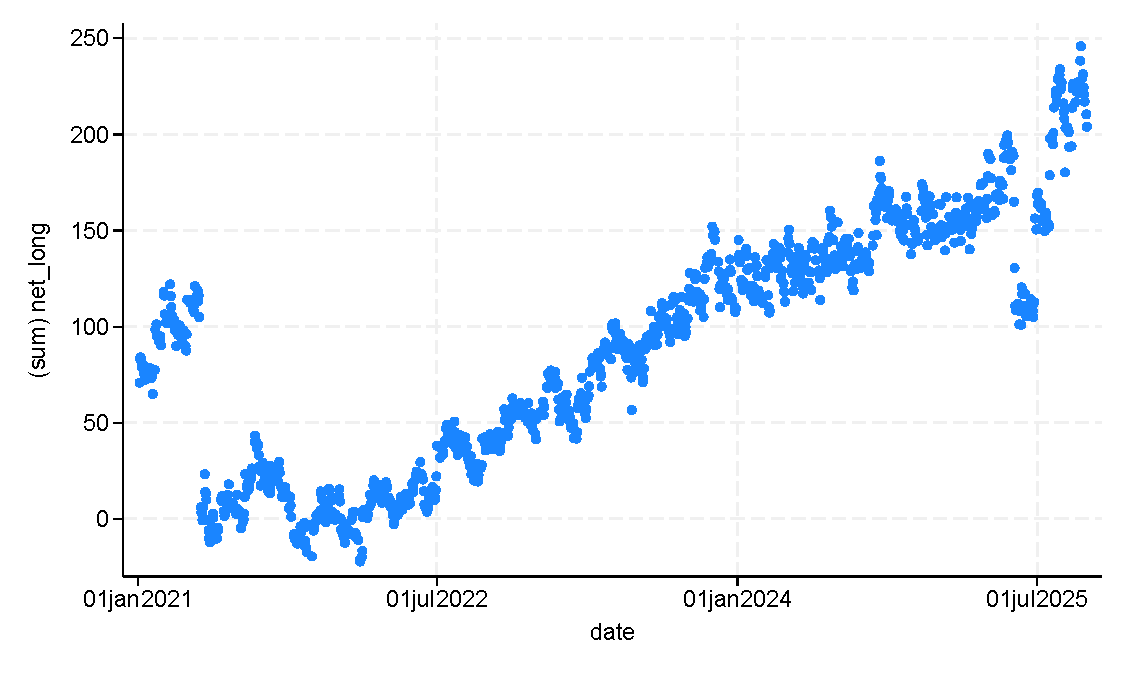
\includegraphics[width=.7\textwidth]{ofrcomp.pdf})
\end{frame}

% ===========================================================================
\section{Anatomy: who, with whom, in what}
\begin{frame}{Anatomy: who, with whom, in what}
  \begin{itemize}
    \item Fund concentration.
    \item Dealer concentration: $>$50\% financed by three dealers.
    \item Bond selection: not CTD, not OTR --- positive Svensson pricing errors, in both jurisdictions.
    \item Interpretation: funds are paid to hold what curve-sensitive investors and dealers don't want --- liquidity and convergence provision in the illiquid segment.
  \end{itemize}
  % TODO: figures/EUR_ctd.png, figures/USD_ctd.png, figures/EUR_otr.png, ...
  % TODO: CTD difference tables (tables/t1.tex, tables/dFV.tex, ...)
\end{frame}

% ===========================================================================
\section{Risk and return of the trade}
\begin{frame}{Risk and return of the trade}
  \begin{itemize}
    \item Duration offset; convexity gap and its dependence on rate volatility and term premium.
    \item P\&L decomposition: pricing-error convergence $+$ carry $+$ repo specialness $-$ financing cost $-$ margin cost.
    \item Output: ex-ante fund--bond-level risk exposure measure (treatment intensity for the fragility tests).
  \end{itemize}
  % TODO: figures/dur1.pdf, figures/dur2.pdf, figures/con1.pdf, figures/con2.pdf
\end{frame}

% ===========================================================================
\section{The funding architecture}
\begin{frame}{The funding architecture}
  \begin{itemize}
    \item Repo terms by fund$\times$dealer pair: rates, haircuts, tenor, rollover frequency.
    \item Relationship stability over time.
    \item Takeaway: funding is concentrated, short-tenor, and relationship-based.
  \end{itemize}
  % TODO: figures/distribution_HF_counterparties.png
\end{frame}

% ===========================================================================
\section{Fragility I: the dealer funding channel}
\begin{frame}{Fragility I: the dealer funding channel}
  \begin{itemize}
    \item Khwaja--Mian design: same fund, multiple dealers, fund$\times$time fixed effects.
    \item Shocks: recurring year-end balance-sheet contractions (power), April 2025 (salience).
    \item Outcomes in sequence: financing quantities $\rightarrow$ position cuts $\rightarrow$ which bonds get cut first (prediction: the cheapest, least liquid).
  \end{itemize}
\end{frame}

% ===========================================================================
\section{Fragility II: the volatility shock and its propagation}
\begin{frame}{Fragility II: the volatility shock and its propagation}
  \begin{itemize}
    \item April 2025 as the realized convexity-gap event; treatment intensity from the ex-ante exposure measure.
    \item Cross-market test: did UST-exposed funds cut EGB positions more, within bond$\times$week?
    \item Spillover: did exposed bonds' prices and liquidity move?
  \end{itemize}
\end{frame}

\begin{frame}{The causal chain}
  \centering
  Dealer or US-book shock\\[.5em]
  $\downarrow$\\[.5em]
  Fund's financing or capital contracts \hfill {\small (dealer funding channel)}\\[.5em]
  $\downarrow$\\[.5em]
  Fund adjusts positions in the other market \hfill {\small (cross-market transmission)}\\[.5em]
  $\downarrow$\\[.5em]
  Bond-level prices and liquidity move with exposure \hfill {\small (spillover result)}
\end{frame}

% ===========================================================================
\section{Implications}
\begin{frame}{Implications}
  \begin{itemize}
    \item The risk is not directional exposure but convexity and funding concentration in illiquid bonds.
    \item Not what current NBFI monitoring measures --- consequences for the transparency and leverage debates.
  \end{itemize}
\end{frame}

% ===========================================================================
\appendix
\section*{Backup}
\begin{frame}{Backup}
  % TODO: robustness figures and tables
\end{frame}

\end{document}
